\documentclass[11pt,a4paper]{article}
\usepackage[T1]{fontenc}
\usepackage[utf8]{inputenc}
\usepackage{amsmath,amssymb}
\usepackage{geometry}
\geometry{margin=1.1in}
\usepackage{graphicx}
\graphicspath{{./}{./figures/}{../dossier/figures/}}
\usepackage{booktabs}
\usepackage[expansion=false]{microtype}
\usepackage{float}
\usepackage[bottom]{footmisc}
\usepackage[colorlinks=true,linkcolor=black,urlcolor=blue!50!black,citecolor=black]{hyperref}
\usepackage{xcolor}
\usepackage{array}
\usepackage{tabularx}
\usepackage{tikz}
\usetikzlibrary{calc}
\usepackage{pgfplots}
\pgfplotsset{compat=1.16}
\usepgfplotslibrary{groupplots}

\definecolor{citecolor}{gray}{0}

\newcommand{\cy}[2]{\hyperlink{cite.#1}{\textcolor{citecolor}{#2}}}
\newcommand{\prot}[1]{\textsf{#1}}
\newcommand{\psale}{\pi^{\mathrm{sale}}}
\newcommand{\sale}{\mathrm{sale}}
\newcolumntype{L}{>{\raggedright\arraybackslash}X}
\setlength{\intextsep}{10pt}
\setlength{\abovecaptionskip}{6pt}
\interfootnotelinepenalty=10000

\title{Same Choices, Different Reasonings:\\ An Explanatory Note on the Experimental Design}
\author{Francesco Pinna \and Emanuele Sebastianelli}
\hypersetup{urlcolor=black, pdftitle={Same Choices, Different Reasonings: An Explanatory Note on the Experimental Design}, pdfauthor={Francesco Pinna and Emanuele Sebastianelli}}
\date{November 2026\thanks{Emails: \href{mailto:francesco.pinna@studenti.luiss.it}{francesco.pinna@studenti.luiss.it} and \href{mailto:e.sebastianelli@studenti.luiss.it}{e.sebastianelli@studenti.luiss.it}. Note prepared for Daniela Di Cagno as part of the course project for Experimental and Behavioural Economics, LUISS Guido Carli, taught by Daniela Di Cagno and Irene Maria Buso, academic year 2026--2027. The design implements the experiment requested by the companion paper, Pinna (2026). We thank Lorenzo Spadoni for his comments at the intermediate presentation of November 11, 2026. All remaining errors are our own.}}

\begin{document}
\maketitle

\begin{abstract}
\noindent A buyer who pays too much for a good of uncertain quality may overestimate its value, or she may neglect what the seller's willingness to sell reveals about it, and the price she offers does not tell the two errors apart. The design described here separates them with two reservation prices for the same good, stated against two computerized sellers whose rules are announced, one who always sells and one who sells more often when the good is worth little. The first price measures the value that the participant attaches to the good, and the distance between the two prices measures how much of the seller's selection she takes into account. Three elicitation protocols, which differ only in the moments at which prices are collected, turn the act of measuring into a treatment, and the note explains task, incentives, controls, hypotheses and sample in the language of experimental practice, with one numerical example that runs through the text.
\end{abstract}

\section{The economic problem and the questions of the design}\label{sec:problem}

The design starts from a problem of asymmetric information, in which a seller knows what a good is worth while the buyer does not, so that the seller's willingness to trade is itself informative, a good of low value being given up more readily than a good of high value. In the market for lemons of \cy{akerlof}{Akerlof (1970)} this mechanism drives the good cars out of the market, and in the laboratory it takes the form of the acquiring-a-company problem of \cy{samuelsonbazerman}{Samuelson and Bazerman (1985)}, where buyers systematically offer more than the firm is worth to them once the acceptance of the offer is taken into account. A buyer who reasons correctly lowers her offer because she understands that a completed trade is bad news about the good.

An offer that is too high can come from two different errors, since the buyer may hold too favorable a belief about the value of the good, for instance because she gives too much weight to an encouraging piece of evidence, or she may hold an accurate belief and fail to draw the inference contained in the seller's behavior. The two errors lead to the same offer and differ in everything that precedes it, namely in the beliefs held along the way and in the reaction to new information, which is the sense of the title of the project and the reason why an experiment that records a single offer cannot tell which of the two produced it.

The design is built around one main question, whether buyers take the seller's selection into account less than a correct inference requires, once their own valuation of the good has been measured separately. Answering it requires decisions taken at intermediate moments, before all the information has arrived, and the design therefore also asks whether such intermediate requests change the final decision, so that the measurement instrument is itself examined as a treatment. Should the neglect of selection be present, the same data allow a comparison between two descriptions of it proposed in the literature.

The exposition follows the order in which a participant meets the experiment, from the task to the payment, accompanied by a numerical example with a prior of 0.4 and the strong rule of selection, while Appendix~\ref{sec:terms} lists the terms and symbols of the note with their usual names in the literature, Appendix~\ref{sec:rules} relates the two descriptions of the neglect to the companion paper, and Appendix~\ref{sec:instructions} reproduces the instructions for participants.

The design is presented in its current state, which differs from the slides of the intermediate presentation of November 11, 2026 in three respects that follow from the discussion held on that occasion. Trials in which each price is stated alone have been added (Section~\ref{sec:pull}), a third and stronger intensity of selection has been introduced in order to compare the two descriptions of the neglect (Section~\ref{sec:form}), and an exploratory guessing game between paired participants, unrelated to the hypotheses, has been removed to make room for the new trials.

\section{Relation to the experimental literature and to the companion paper}

The closest antecedent in the environment of this course is the acquiring-a-company experiment of \cy{dicagno}{Di Cagno, G\"uth, Lohse, Marazzi and Spadoni (2024)}, in which a seller who knows the value of the firm sends a message about it to the buyer, the buyer proposes a price that the seller accepts or rejects, and with a known probability a leak reveals the true value to the buyer. That design studies the whole strategic relation, with its mixture of beliefs about the other party, attitudes toward misreporting and inference from the other party's behavior, whereas the present one isolates a single component of it. The seller is replaced by a computer whose rule is announced, as in \cy{charnesslevin}{Charness and Levin (2009)}, who show that the overbidding of the acquiring-a-company problem survives when the problem is reduced to an individual decision without a human counterpart. The decision of the computerized seller to sell plays the role that the acceptance of the offer plays in that game and in their version of it, with the difference that it does not depend on the price, so that the selection faced by the buyer is the same whatever she states. With a programmed seller the buyer has nothing to guess about intentions or honesty, the correct inference has a closed form, and any distance between behavior and benchmark can be attributed to the treatment of the information contained in the sale, at the price of a design that is silent on the strategic side of the problem.

The error of interest is the one that \cy{eysterrabin}{Eyster and Rabin (2005)} attribute to a cursed player, who underestimates the dependence of other players' actions on their private information, and that they index by a number between zero and one, called here the degree of selection neglect. \cy{espondavespa}{Esponda and Vespa (2014)} trace similar failures to the difficulty of reasoning on hypothetical events, \cy{ngangoue}{Ngangou\'e and Weizs\"acker (2021)} document that traders learn less from a price they have to imagine than from one they observe, and \cy{enke}{Enke (2020)} finds that many subjects neglect the selection behind the data they see. The present task is closest to these settings, where the informative event does not respond to the subject's choice, whereas in the acquiring-a-company problem the buyer's own offer decides which goods she obtains. To this evidence our measure adds a quantity in points on a price scale, separated from the participant's belief about the good and observable at several moments of the same decision.

On the side of measurement, the design belongs to the methods surveyed by \cy{schlag}{Schlag, Tremewan and van der Weele (2015)} that infer beliefs from choices and never ask for a probability. \cy{danz}{Danz, Vesterlund and Wilson (2022)} show that reports under the binarized scoring rule are pulled toward the center, the more so when the incentives are explained in detail, and a report flattened toward the center would be indistinguishable from the neglect under study. Beliefs are therefore read from purchase decisions on a price list paid with the mechanism of \cy{bdm}{Becker, DeGroot and Marschak (1964)}, a format whose own framing effects, documented by \cy{andersen}{Andersen, Harrison, Lau and Rutstr\"om (2006)}, are addressed by the controls of Section~\ref{sec:threats}. The question of whether the act of eliciting changes behavior belongs to the literature surveyed by \cy{brandts}{Brandts and Charness (2011)}, and here it is answered with a test of equivalence in the sense of \cy{schuirmann}{Schuirmann (1987)}.

According to the companion paper, \cy{pinna}{Pinna (2026)}, whose results can be stated here without their mathematics, final choices alone cannot separate noisy responses, neglect of selection and limited depth of reasoning, because these mechanisms can produce the same choices and differ in the beliefs held before them. Beliefs recorded along the way restore the separation, since a correct belief moves only when information arrives, whereas a belief distorted by neglect departs from it in a predictable direction. A record taken along the way can however alter what it records, and the paper therefore asks for an experiment with a randomized timing of the intermediate measurements, with one uninterrupted group, and with an estimate of the noise of the instrument from repeated measurements at unchanged information. The three protocols of Section~\ref{sec:protocols} and the lists with an announced value of Section~\ref{sec:threats} implement that request, and nothing else of that paper is needed to read what follows.

\section{The purchase task}\label{sec:task}

\subsection{The good and the information about its value}

In every trial there is a single good, worth either 30 or 90 points, and the participant is told the prior probability that it is worth 90, which is 0.4 in half of the trials and 0.6 in the other half. During the trial she receives two certificates about the value, generated independently of each other given the true value, one of which reports the true value in 70 percent of cases and the other in 60 percent, with the accuracies displayed and the order of arrival drawn at random. Neither certificate settles the question, and this is deliberate, because a buyer who became almost certain of the value would state nearly the same price for any seller and the selection would leave no trace in the data.

The correct belief follows from Bayes' rule, which is most simply applied in terms of odds, since a certificate that reads high multiplies the odds of the value 90 by 7/3 when it is the more accurate one and by 3/2 when it is the less accurate one, while a certificate that reads low multiplies them by 3/7 and by 2/3 respectively. From a prior of 0.4, that is, from odds of 2 to 3, two certificates that read low give odds of 4 to 21 and a probability of 0.16, and Table~\ref{tab:posteriors} reports the correct belief after both certificates in every case. This final belief does not depend on the order of arrival, whereas the belief held after the first certificate does, so that the random order generates different paths toward the same final information.

\begin{table}[H]
\centering
\begin{tabular}{@{}llcc@{}}
\toprule
Certificate with accuracy 0.70 & Certificate with accuracy 0.60 & Prior 0.4 & Prior 0.6\\
\midrule
reads high & reads high & 0.70 & 0.84\\
reads high & reads low & 0.51 & 0.70\\
reads low & reads high & 0.30 & 0.49\\
reads low & reads low & 0.16 & 0.30\\
\bottomrule
\end{tabular}
\caption{Correct probability that the good is worth 90 after both certificates.}
\label{tab:posteriors}
\end{table}

\subsection{The two computerized sellers}

The same good is offered by two sellers, both played by the computer according to rules that the participant reads before deciding, and while Seller~1 always sells, Seller~2 is selective, since the probability with which it sells is higher when the good is worth 30, exactly as an informed owner parts more willingly with a bad good. The rule of Seller~2 changes across trials among the three intensities of Table~\ref{tab:sellers}, and in a few control trials it is replaced by a placebo rule that sells with probability one half whatever the value, while in no case does the decision to sell depend on the price or on the answers of the participant. The two sellers are alternative counterparts for the same good, of which at most one purchase is implemented at the end of the session, and since they follow the announced rules and nothing in the task is concealed or misrepresented, the design involves no deception.

\begin{table}[H]
\centering
\begin{tabular}{@{}lcc@{}}
\toprule
Seller & Sells if the good is worth 30 & Sells if the good is worth 90\\
\midrule
Seller 1, always available & 1 & 1\\
Seller 2, weak selection & 0.65 & 0.35\\
Seller 2, strong selection & 0.80 & 0.20\\
Seller 2, very strong selection & 0.95 & 0.05\\
Placebo seller & 0.50 & 0.50\\
\bottomrule
\end{tabular}
\caption{Announced rules of the computerized sellers, as probabilities of selling.}
\label{tab:sellers}
\end{table}

\subsection{The reservation price and the price list}

For each seller the participant states her reservation price, the highest price at which she is willing to buy from that seller, on a list of 71 prices in steps of one point. She types a threshold in a field showing the range of allowed prices, the screen marks as purchases all the prices up to it and as refusals all those above, and she confirms after seeing the summary, with no value preselected and the possibility of refusing or buying at every price, as in Figure~\ref{fig:facsimile}.

\begin{figure}[H]
\centering
\begin{tikzpicture}
\node[anchor=south west, inner sep=0pt] (img) at (0,0) {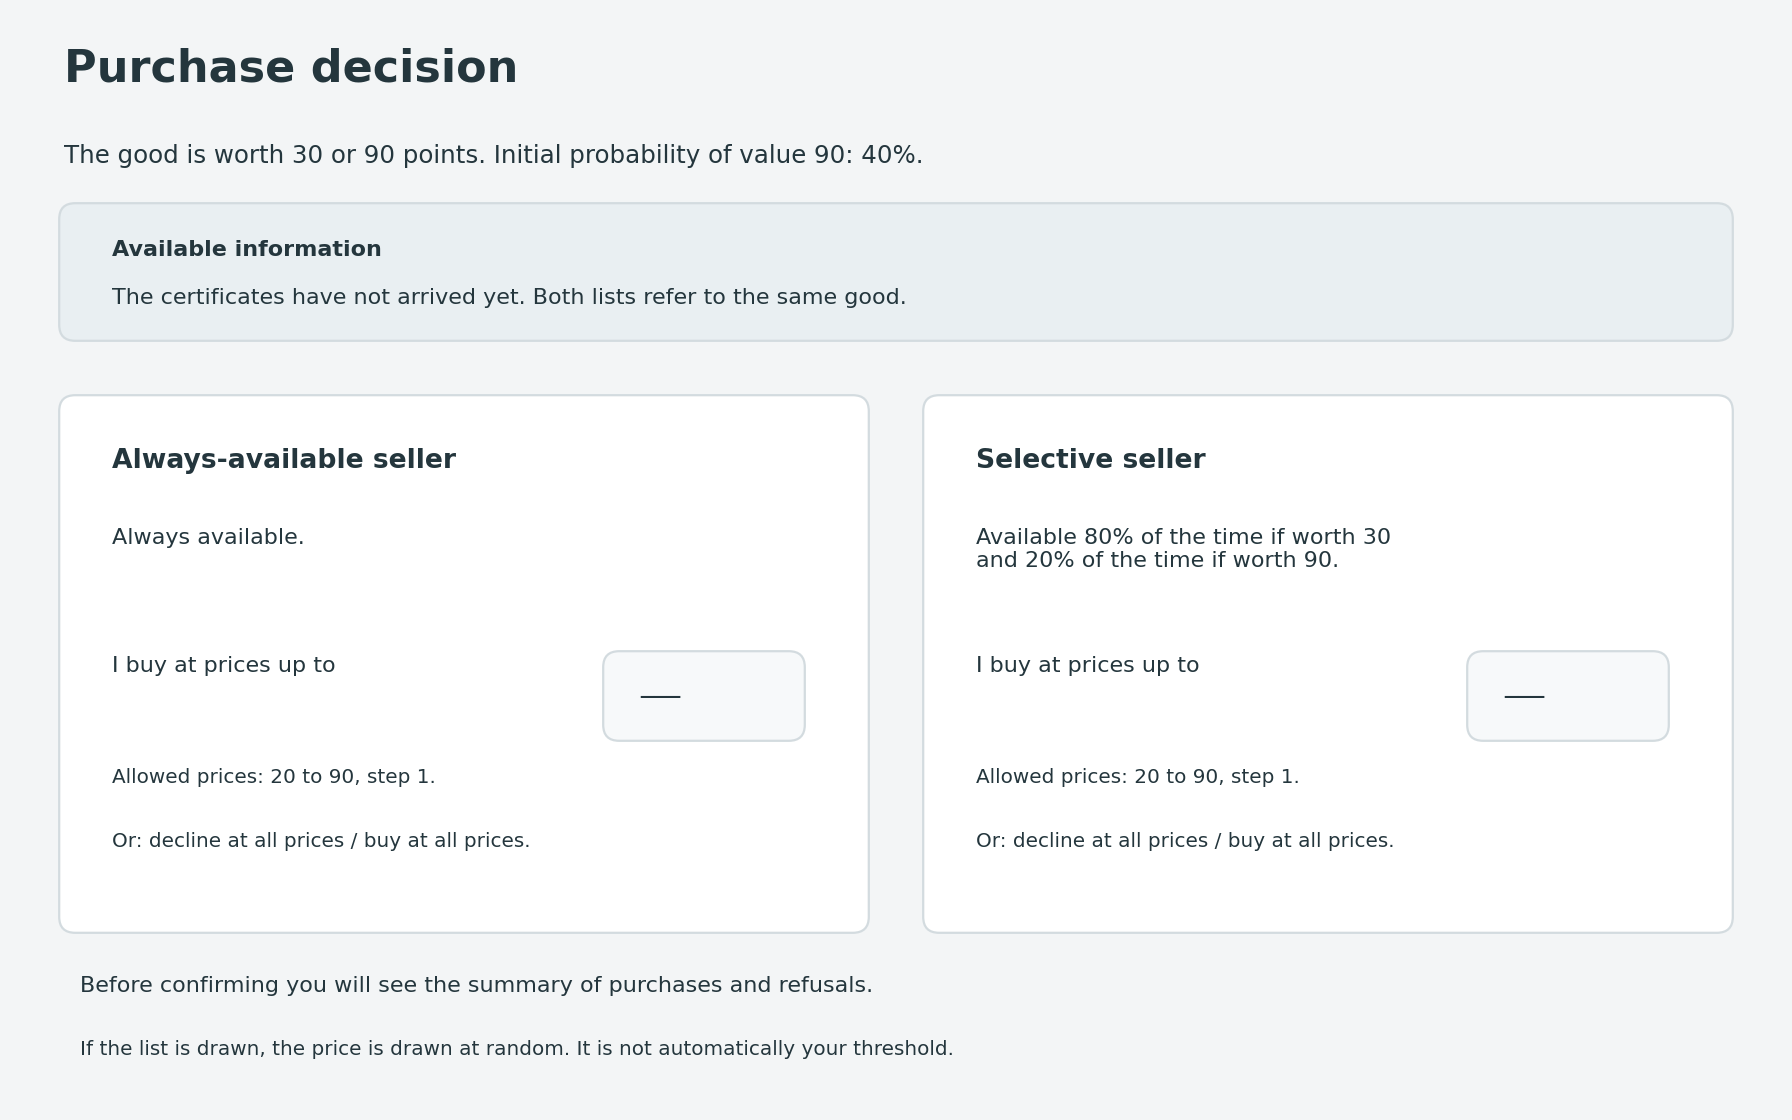
\includegraphics[width=0.66\linewidth]{facsimile_X.png}};
\begin{scope}[x={(img.south east)}, y={(img.north west)}, black!60, line width=0.4pt, rounded corners=1.6pt]
\draw (0.033203,0.695982) rectangle (0.966797,0.818304);
\draw (0.032924,0.166964) rectangle (0.484933,0.647321);
\draw (0.515067,0.166964) rectangle (0.967076,0.647321);
\draw (0.336496,0.338393) rectangle (0.449219,0.418750);
\draw (0.818638,0.338393) rectangle (0.931362,0.418750);
\end{scope}
\draw[black!60, line width=0.4pt] (img.south west) rectangle (img.north east);
\end{tikzpicture}
\caption{Facsimile of the purchase screen at the beginning of a trial, before the certificates arrive, with Seller~1 on the left and Seller~2 on the right. No threshold is preselected. The image illustrates the task and is not a working application.}
\label{fig:facsimile}
\end{figure}

The list is paid with the mechanism of \cy{bdm}{Becker, DeGroot and Marschak (1964)}, under which, if a list is selected for payment, the computer draws one of its 71 prices with equal probability and applies the decision stated for that price. Nothing happens when the drawn price is above the threshold, whereas when it is at or below the threshold the participant buys at the drawn price, provided the seller sells, and her result in points is the value of the good minus the drawn price, so that the threshold itself is never the price paid. A threshold above the true reservation price exposes the participant to purchases she would prefer to avoid, a threshold below it gives up purchases she would like to make, and stating the true reservation price is therefore a weakly dominant strategy, for the same reason for which bidding one's value is dominant in the second-price auction of \cy{vickrey}{Vickrey (1961)}.

The list comes in two formats, from 20 to 90 and from 30 to 100, assigned at random and in equal numbers to the trials of each participant. Every reservation price that the reasoning studied here can justify lies between 30 and 90, so that both formats contain all the relevant prices. The ten additional prices, placed below in one format and above in the other, leave room for mistakes outside that range, and they move the center of the list from 55 to 65 without changing anything of economic substance, which makes it possible to detect a tendency to answer toward the middle of whatever list is shown.

\section{From two prices to a measure of selection neglect}\label{sec:measure}

\subsection{The two benchmark prices}

Let $\pi$ denote the probability that the participant assigns to the value 90 given the information seen so far, a number between zero and one. Since Seller~1 always sells, the good bought from it is worth 90 with probability $\pi$, and the correct reservation price is the expected value
\[
U(\pi)\;=\;30+60\,\pi .
\]
A purchase from Seller~2 takes place only when Seller~2 sells, and since the fact that it sells is informative, the relevant belief is the probability that the good is worth 90 given, in addition, that Seller~2 sells, which we denote by $\psale$ and which by Bayes' rule equals
\[
\psale\;=\;\frac{\pi\,\Pr(\sale\mid 90)}{\pi\,\Pr(\sale\mid 90)+(1-\pi)\,\Pr(\sale\mid 30)},
\]
a number smaller than $\pi$ whenever the seller is selective. The price matters only if the purchase takes place, and the correct reservation price for Seller~2 is therefore the expected value of the good conditional on the sale,
\[
C(\pi)\;=\;30+60\,\psale .
\]
With a belief of 0.4 and strong selection, a sale multiplies the odds of the value 90 by $0.20/0.80$, so that $\psale$ equals $1/7$, the benchmark prices are $U=54.00$ and $C=38.57$, and a buyer who reasons correctly pays Seller~2 about fifteen points less than Seller~1.

\subsection{The price of a buyer who neglects part of the selection}

A buyer who neglects the selection entirely treats a sale by Seller~2 as uninformative and states for it the same price as for Seller~1, and \cy{eysterrabin}{Eyster and Rabin (2005)} describe the intermediate cases with a single number $\chi$ between zero and one, the degree of selection neglect, which they call cursedness. A buyer with degree $\chi$ reasons as if the decision to sell were unrelated to the value with probability $\chi$ and correctly related to it with probability $1-\chi$, so that the probability she assigns to the value 90 after a sale is the average $(1-\chi)\,\psale+\chi\,\pi$.\footnote{In the definition of \cy{eysterrabin}{Eyster and Rabin (2005)} the buyer attributes to the seller, at either value $v$ of the good, the selling probability $(1-\chi)\Pr(\sale\mid v)+\chi\Pr(\sale)$, an average of the announced rule and of the overall probability of a sale, and Bayes' rule applied to this perceived rule returns the average in the text.} Since the reservation price is linear in this probability, her price for Seller~2 is
\[
S(\pi,\chi)\;=\;C(\pi)+\chi\,\bigl[U(\pi)-C(\pi)\bigr],
\]
a point on the segment between the correct price $C$ and the price $U$ of complete neglect, at a fraction $\chi$ of the way. In the example, a degree of neglect of 0.25 gives $S=38.57+0.25\times 15.43=42.43$, and Table~\ref{tab:benchmarks} reports the benchmark prices for the three rules of Seller~2.

\begin{table}[H]
\centering
\begin{tabular}{@{}lccccc@{}}
\toprule
Rule of Seller 2 & $\psale$ & $C$ & $U-C$ & $S$ with $\chi=0.25$ & $S$ with $\chi=0.50$\\
\midrule
Weak selection & 0.264 & 45.85 & 8.15 & 47.89 & 49.92\\
Strong selection & 0.143 & 38.57 & 15.43 & 42.43 & 46.29\\
Very strong selection & 0.034 & 32.03 & 21.97 & 37.53 & 43.02\\
\bottomrule
\end{tabular}
\caption{Benchmark prices in points at a belief of 0.4, for which $U=54.00$ under every rule.}
\label{tab:benchmarks}
\end{table}

\subsection{The degree of neglect implied by a pair of stated prices}

Read backwards, the identity recovers the degree of neglect from the two prices that a participant states for Seller~1 and for Seller~2 on the same information, which we denote by $P_1$ and $P_2$. The first price reveals the belief she holds about the good, $\hat\pi=(P_1-30)/60$, whether or not that belief is correct, and from this belief one computes the price $C(\hat\pi)$ that a correct inference about Seller~2 would imply for her, so that the degree of neglect is the share of the distance between her first price and this price that she fails to cover,
\[
\hat\chi\;=\;\frac{P_2-C(\hat\pi)}{P_1-C(\hat\pi)} .
\]
A participant who states 54 and 42.43 thus reveals a belief of 0.4 and a degree of neglect of 0.25. The use of the belief revealed by the first price, in place of the correct belief computed by the experimenter, is what separates the two errors of Section~\ref{sec:problem}, since a participant who misreads the certificates states a first price that differs from the benchmark and her mistake is absorbed by $\hat\pi$ without being counted as neglect. The ratio conveys the logic of the measure, while the estimate itself combines all the trials of a participant in the statistical model of Section~\ref{sec:hypotheses}, because a single pair of prices is observed with noise and on a grid of one point.

\section{A complete trial followed step by step}\label{sec:example}

Table~\ref{tab:example} follows a participant through a trial in which both sellers are priced at the three moments of the trial, as in the richest of the protocols of Section~\ref{sec:protocols}. The prior is 0.4, Seller~2 follows the strong rule, the more accurate certificate arrives first and both certificates read low, while the stated prices are those of a hypothetical buyer who updates her belief correctly, neglects one third of the selection and answers on the list of whole prices.

\begin{table}[H]
\centering
\small
\begin{tabular}{@{}llccccc@{}}
\toprule
Seconds & Information on the screen & $\pi$ & $U$ & $C$ & Stated $P_1$, $P_2$ & $\hat\chi$\\
\midrule
10 to 40 & prior and rule of Seller 2 & 0.40 & 54.00 & 38.57 & 54, 43 & 0.29\\
60 to 90 & first certificate reads low & 0.22 & 43.33 & 34.00 & 43, 37 & 0.34\\
120 to 150 & second certificate reads low & 0.16 & 39.60 & 32.73 & 39, 35 & 0.38\\
\bottomrule
\end{tabular}
\caption{A trial with prior 0.4 and strong selection. The columns $\pi$, $U$ and $C$ are the correct belief and the benchmark prices, and $\hat\chi$ is computed from the stated prices as in Section~\ref{sec:measure}.}
\label{tab:example}
\end{table}

The certificates lower the correct belief from 0.40 to 0.22 and then to 0.16, and both benchmark prices fall with it, while the stated price for Seller~1 tracks $U$, which shows that this participant reads the certificates correctly, and the stated price for Seller~2 stays above $C$ at every moment. Computed from these thresholds, the share of the gap that she fails to cover moves between 0.29 and 0.38 although the buyer neglects one third throughout, only because a threshold is the highest whole price that does not exceed the reservation price. A single pair of prices is therefore a coarse measurement, and the final pair alone is compatible with any degree of neglect between 0.30 and 0.54.

Suppose that at the end of the session the final list for Seller~2 of this trial is selected for payment and the computer draws the price 33, which is below the stated threshold of 35, so that the participant buys if Seller~2 sells. The good is worth 30, Seller~2 sells with probability 0.80 and does sell, and the result is $30-33=-3$ points, which lowers the probability of winning the prize from 50 to 47.9 percent according to the rule of Section~\ref{sec:session}. Conditional on a sale the good was worth 32.73 points in expectation, so that a threshold of 35 accepts three prices, 33, 34 and 35, at which purchases lose points on average and which a buyer who had drawn the correct inference would have refused.

\section{Threats to the interpretation of the prices and controls}\label{sec:threats}

A gap between the two stated prices that is smaller than the gap $U-C$ can have causes other than the neglect of selection, and for each of the main alternatives the design contains a variation that distinguishes it from the neglect or measures it, according to the correspondence that Table~\ref{tab:threats} summarizes at the end of the section.

\subsection{Attraction toward the center of the price list}

Answers on a price list tend toward its middle, as \cy{andersen}{Andersen, Harrison, Lau and Rutstr\"om (2006)} discuss for lists displayed row by row, and a threshold typed against a declared range may do the same, which imitates the neglect because it compresses the two prices toward each other. A buyer who draws the correct inference and moves each price by 10 percent of its distance from the center would display, at a belief of 0.4 and under strong selection, an apparent neglect of 0.10 with the center at 55 and of 0.13 with the center at 65, nearly the same under the three intensities, so that comparing them does not expose the artifact.

The design measures the attraction through the two formats of the list, whose centers are ten points apart, since a buyer attracted by the center with a weight of 10 percent states prices that differ by one point between the formats, whereas the neglect does not depend on the format. A second measure comes from eight additional lists that announce the value of the good, equal to 36, 48, 66 or 78 points and presented once in each format, in which the correct reservation price is the announced value for both sellers and any systematic departure from it is a property of the instrument, and the attraction estimated from these two sources enters the statistical model as a separate component.

\subsection{Dependence between two prices stated on the same screen}\label{sec:pull}

When the two prices are stated side by side, the second may be obtained by adjusting the first, and since adjustments from an initial value are typically insufficient, as in the anchoring and adjustment heuristic of \cy{tversky}{Tversky and Kahneman (1974)}, the gap between the two prices of the same person would be too small even for a buyer who understands the selection perfectly. This dependence, pointed out by Lorenzo Spadoni at the intermediate presentation, has a precise consequence for the design, which is best stated by letting $\kappa$ denote the share of her own gap that a participant closes when she states the two prices together, a number between zero and one that we call the pull. Under the averaging rule of Section~\ref{sec:measure}, the price stated for Seller~2 in a joint statement corresponds to a degree of neglect of
\[
\chi+\kappa\,(1-\chi),
\]
so that two prices stated on the same screen identify only this combination, and a buyer with no neglect and a pull of 0.10 is indistinguishable, on such data, from a buyer with a neglect of 0.10 and no pull.\footnote{Stated alone, the price for Seller~2 is $S=C+\chi\,(U-C)$, and the joint statement moves it toward $U$ by a share $\kappa$ of their distance, to $S+\kappa\,(U-S)=C+[\chi+\kappa\,(1-\chi)]\,(U-C)$. Under the dampening rule the same holds with $\chi$ replaced by the share of $U-C$ left uncovered when Seller~2 is priced alone.}

The design separates the two by adding trials in which each price is stated alone, for which participants are grouped in pairs with common draws. In a single-seller trial the two members of a pair face the same good, the same prior and the same certificates, while one states a price only for Seller~1 and the other only for Seller~2, with roles that alternate across trials and without interaction or view of each other's answers. The pull cannot operate in these trials, because no participant has a first price of her own to adjust, so that the gap between the two prices, which the joint trials measure within a person, is here measured between two persons who hold the same evidence, and if joint statements compress the gap, the first measure is smaller than the second on average. Differences in beliefs between partners add noise to the second measure without biasing it, since roles are assigned at random.

\subsection{The functional form of the neglect}\label{sec:form}

The averaging rule of \cy{eysterrabin}{Eyster and Rabin (2005)} describes a buyer in doubt about the seller, who reads the sale correctly with probability $1-\chi$ and as no news at all with probability $\chi$. The experimental literature on belief updating, from \cy{grether}{Grether (1980)} to the survey of \cy{benjamin}{Benjamin (2019)}, describes insufficient inference in another way, as the behavior of a person who has no doubt about the direction of the news and takes every piece of evidence to be weaker than it is. Applied to the sale, this dampening rule describes a buyer who treats the seller as less selective than announced, so that with a degree of one half the strong rule, under which a good worth 30 is four times as likely to be sold as a good worth 90, counts for her as a rule under which it is twice as likely.\footnote{In terms of odds, the buyer multiplies the odds $\pi/(1-\pi)$ of the value 90 by the likelihood ratio of the sale, $\Pr(\sale\mid 90)/\Pr(\sale\mid 30)$, raised to the power $1-\chi$, and prices the good accordingly.} The two rules coincide when the neglect is absent and when it is complete and differ in between, as Figure~\ref{fig:rules} shows for the three intensities.

\begin{figure}[H]
\centering
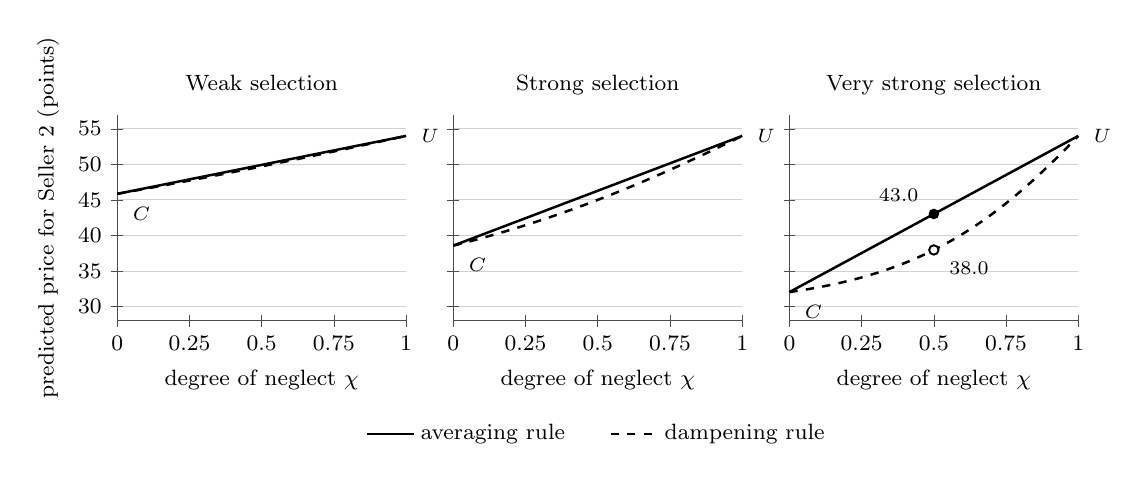
\begin{tikzpicture}[declare function={
  corr(\r)=30+60*((2/3)*\r)/(1+(2/3)*\r);
  aver(\x,\r)=corr(\r)+\x*(54-corr(\r));
  damp(\x,\r)=30+60*((2/3)*(\r)^(1-\x))/(1+(2/3)*(\r)^(1-\x));
}]
\begin{groupplot}[
  group style={group size=3 by 1, horizontal sep=0.6cm, ylabels at=edge left, yticklabels at=edge left},
  width=5.25cm, height=4.2cm,
  xmin=0, xmax=1, ymin=28, ymax=57,
  xtick={0,0.25,0.5,0.75,1}, xticklabels={0,0.25,0.5,0.75,1},
  ytick={30,35,40,45,50,55},
  xlabel={degree of neglect $\chi$},
  tick label style={font=\footnotesize}, label style={font=\footnotesize}, title style={font=\footnotesize, yshift=-3pt, text height=1.6ex, text depth=0.5ex},
  axis lines=left, axis line style={-, black!70}, tick style={black!70},
  ymajorgrids, grid style={black!18, line width=0.3pt},
  domain=0:1, samples=81, clip=false]
\nextgroupplot[title={Weak selection}, ylabel={predicted price for Seller 2 (points)},
  legend to name=ruleslegend, legend columns=2,
  legend style={draw=none, font=\footnotesize, /tikz/every even column/.append style={column sep=1.4em}}]
\addplot[black, line width=0.9pt] {aver(x,0.35/0.65)};
\addlegendentry{averaging rule}
\addplot[black, line width=0.9pt, dashed] {damp(x,0.35/0.65)};
\addlegendentry{dampening rule}
\node[font=\scriptsize, anchor=west] at (axis cs:1.02,54) {$U$};
\node[font=\scriptsize, anchor=north west] at (axis cs:0.02,45.4) {$C$};
\nextgroupplot[title={Strong selection}]
\addplot[black, line width=0.9pt] {aver(x,0.20/0.80)};
\addplot[black, line width=0.9pt, dashed] {damp(x,0.20/0.80)};
\node[font=\scriptsize, anchor=west] at (axis cs:1.02,54) {$U$};
\node[font=\scriptsize, anchor=north west] at (axis cs:0.02,38.1) {$C$};
\nextgroupplot[title={Very strong selection}]
\addplot[black, line width=0.9pt] {aver(x,0.05/0.95)};
\addplot[black, line width=0.9pt, dashed] {damp(x,0.05/0.95)};
\addplot[only marks, mark=*, mark size=1.7pt, black] coordinates {(0.5,43.02)};
\addplot[only marks, mark=*, mark size=1.7pt, black, mark options={fill=white, line width=0.7pt}] coordinates {(0.5,37.96)};
\node[font=\scriptsize, anchor=south east] at (axis cs:0.48,43.4) {43.0};
\node[font=\scriptsize, anchor=north west] at (axis cs:0.52,37.6) {38.0};
\node[font=\scriptsize, anchor=west] at (axis cs:1.02,54) {$U$};
\node[font=\scriptsize, anchor=north west] at (axis cs:0.02,31.6) {$C$};
\end{groupplot}
\node[anchor=north] at ($(group c2r1.south)+(0,-1.05cm)$) {\pgfplotslegendfromname{ruleslegend}};
\end{tikzpicture}
\caption{Price predicted for Seller~2 under the two rules at a belief of 0.4, from the correct price $C$ at $\chi=0$ to $U=54$ at $\chi=1$. The dots mark the predictions at $\chi=0.5$.}
\label{fig:rules}
\end{figure}

The two descriptions part ways when the selection becomes extreme, since under the averaging rule the buyer fails to cover the same share $\chi$ of the gap $U-C$ whatever the intensity, whereas under the dampening rule strong evidence gets through even when it is discounted, so that at a belief of 0.4 the share left uncovered by a buyer with a degree of 0.5 falls from 0.47 under weak selection to 0.42 under strong selection and to 0.27 under very strong selection. This is the reason for the third intensity of Table~\ref{tab:sellers}, the first two serving to determine the degree of neglect and the third to discriminate between the forms, a question of little weight for the main hypothesis, since the two rules coincide without neglect.

The design does not choose between the two descriptions in advance, and the analysis that we intend to implement, if the time limits of the course project allow, estimates together with the degree of neglect a weight between zero and one, the rule weight, which is zero when the share left uncovered is the same at all intensities, as under the averaging rule, and one when it falls as the dampening rule predicts. The simpler analysis is the case of a zero weight, under which the first hypothesis is tested, and the cost of one more quantity to estimate and to simulate explains the proviso on time, the averaging formula being the fallback.

We regard the richer analysis as the better one because the averaging formula builds an untested assumption into the measure, and if buyers discount the evidence it reports a degree of neglect that changes with the intensities chosen by the experimenter, lower where the selection is stronger, whereas the rule weight lets the degree keep the same meaning in every trial. The two rules also disagree on where buyers are most exposed, since at a belief of 0.4 the reservation price of a buyer with a degree of 0.5 exceeds the correct one by 4.1, 7.7 and 11.0 points at the three intensities under the averaging rule, and by 12 points against a seller who never parted with a good worth 90, whereas under the dampening rule the excess is 3.9, 6.4 and 5.9 points and vanishes in that limit. The dampening rule, moreover, measures the neglect on the scale on which the statistical model measures the use of the certificates, that of the regressions of \cy{grether}{Grether (1980)}, so that the weight given to the sale can be compared with that of a certificate and a neglect specific to the seller's selection told apart from a general underuse of evidence, while Appendix~\ref{sec:rules} relates both rules to the companion paper.

\subsection{Flat incentives near the optimum}\label{sec:flat}

The mechanism of Becker, DeGroot and Marschak makes the true reservation price optimal, and it punishes small departures from it very lightly, the flat maximum that \cy{harrison}{Harrison (1989)} pointed out for laboratory auctions. A participant who states for Seller~1 a threshold five points above her reservation price loses, in expectation, about a fifth of a point when that list is paid, because she buys at five prices out of 71 that she should have refused and loses between one and five points on each, and with incentives of this size systematic habits such as a cautious understatement of every price can survive.\footnote{A threshold that exceeds a whole reservation price by $d$ points costs $d(d+1)/142$ points in expectation when the list is paid, since the draw is uniform over the 71 prices, and one that falls short of it by $d$ points costs $d(d-1)/142$. The loss thus grows with the square of the departure, as under a quadratic scoring rule on the probability implied by the threshold, and for $d=5$ it equals 0.21 points, that is, 0.15 percentage points of the probability of the prize.}

The design does not remove the problem and responds to it with the steepest linear conversion of points into the probability of the prize that keeps it between zero and one, described in Section~\ref{sec:session}. Before the paid part the participants complete unpaid practice lists after which the drawn price and the outcome are shown, a precaution suggested by the evidence of \cy{casonplott}{Cason and Plott (2014)} that the mechanism is frequently mistaken for one in which the stated price is the price paid. The lists with an announced value measure for each participant the average distance between the stated threshold and the correct one, which the model treats as an individual tendency to understate or overstate, separate from the neglect.

\subsection{Placebo and revelation trials}

Two further kinds of trial check that the gap between the prices responds to the selection and to nothing else, the first of which uses the placebo seller, whose sale is unrelated to the value, so that the two benchmark prices coincide for any degree of neglect and a gap between the stated prices can only come from the instrument. In the revelation trials the participant is told, before the final decision, whether Seller~2 sells, so that the event on which she had to reason hypothetically becomes an observed fact and, if Seller~2 sells, the correct price is the same for both sellers and equal to $C$. The comparison with the ordinary trials shows how much of the neglect is tied to the hypothetical nature of the event, the distinction emphasized by \cy{espondavespa}{Esponda and Vespa (2014)} and by \cy{ngangoue}{Ngangou\'e and Weizs\"acker (2021)}.

\begin{table}[H]
\centering
\small
\begin{tabularx}{\linewidth}{@{}lL@{}}
\toprule
Threat or alternative reading & Element of the design that addresses it\\
\midrule
Attraction toward the center of the list & Two list formats, lists with an announced value\\
Insufficient adjustment between joint prices & Single-seller trials within pairs\\
Misreading of the certificates & Belief revealed by the price for Seller~1\\
Dampening in place of averaging & Third intensity of selection\\
Weak incentives and understatement & Steeper prize rule, practice, understatement term\\
Insensitivity to the probability of the prize & Urn choices (Section~\ref{sec:session})\\
A gap unrelated to the selection & Placebo trials\\
Neglect tied to hypothetical reasoning & Revelation trials\\
\bottomrule
\end{tabularx}
\caption{Threats to the interpretation of the price gap and corresponding controls.}
\label{tab:threats}
\end{table}

\section{Measurement as a treatment, the three elicitation protocols}\label{sec:protocols}

Every trial lasts 150 seconds and follows the same calendar for all participants, in which the prior and the rule of Seller~2 are shown at the start, the first certificate arrives after 50 seconds, the second after 105 seconds, and from second 120 to second 150 every participant takes the final decision. The calendar contains two earlier windows of thirty seconds, one before any certificate and one between the two certificates, a length that the pilot may raise to 45 seconds (Section~\ref{sec:sample}), and the three protocols differ only in the use of these windows, as Figure~\ref{fig:timeline} shows. In protocol \prot{F} no price is requested before the final decision, in protocol \prot{S} prices are requested in one of the two windows, chosen at random for each trial and balanced over priors and intensities, and in protocol \prot{R} prices are requested in both. A window that is not used remains on the screen as waiting time, with the information visible, so that the length of the trial and the time available for thinking are the same in the three protocols.

\begin{figure}[H]
\centering
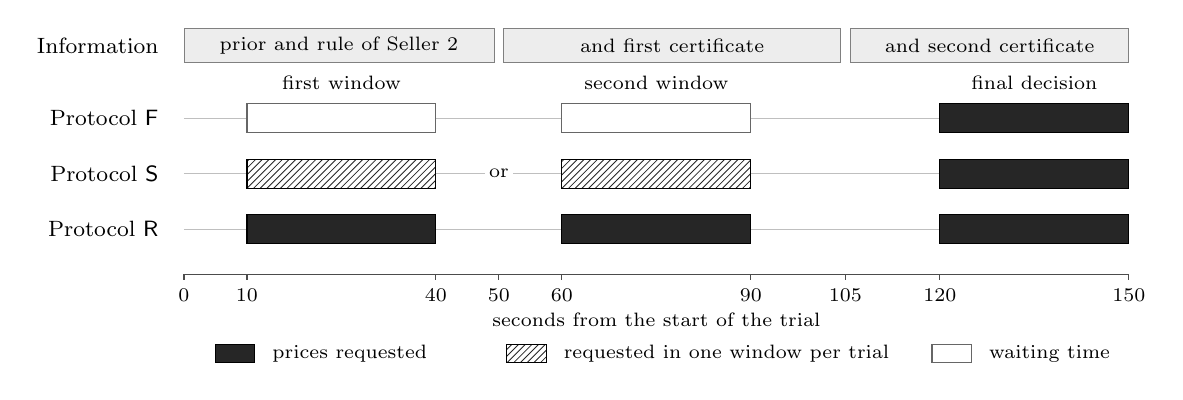
\begin{tikzpicture}[x=0.08cm, y=0.88cm, font=\footnotesize,
  asked/.style={draw=black, line width=0.4pt, fill=black!85},
  idle/.style={draw=black!60, line width=0.4pt, fill=white}]
\def\h{0.21}
\newcommand{\hatched}[4]{\fill[white] (#1,#2) rectangle (#3,#4);
\begin{scope}
  \clip (#1,#2) rectangle (#3,#4);
  \foreach \k in {-8,...,32}{\draw[black!85, line width=0.3pt] ($(#1,#2)+(\k*0.085cm,0cm)$) -- ++(0.6cm,0.6cm);}
\end{scope}
\draw[black, line width=0.4pt] (#1,#2) rectangle (#3,#4);}
\draw[black!50, line width=0.3pt, fill=black!7] (0,3.55) rectangle (49.25,4.05);
\draw[black!50, line width=0.3pt, fill=black!7] (50.75,3.55) rectangle (104.25,4.05);
\draw[black!50, line width=0.3pt, fill=black!7] (105.75,3.55) rectangle (150,4.05);
\node[font=\scriptsize] at (24.6,3.8) {prior and rule of Seller 2};
\node[font=\scriptsize] at (77.5,3.8) {and first certificate};
\node[font=\scriptsize] at (127.9,3.8) {and second certificate};
\node[anchor=east] at (-2.5,3.8) {Information};
\foreach \y/\name in {2.75/F, 1.95/S, 1.15/R}{
  \node[anchor=east] at (-2.5,\y) {Protocol \textsf{\name}};
  \draw[black!25, line width=0.3pt] (0,\y) -- (150,\y);
}
\draw[idle] (10,2.75-\h) rectangle (40,2.75+\h);
\draw[idle] (60,2.75-\h) rectangle (90,2.75+\h);
\draw[asked] (120,2.75-\h) rectangle (150,2.75+\h);
\hatched{10}{1.95-\h}{40}{1.95+\h}
\hatched{60}{1.95-\h}{90}{1.95+\h}
\node[font=\scriptsize, fill=white, inner sep=1.5pt] at (50,1.95) {or};
\draw[asked] (120,1.95-\h) rectangle (150,1.95+\h);
\draw[asked] (10,1.15-\h) rectangle (40,1.15+\h);
\draw[asked] (60,1.15-\h) rectangle (90,1.15+\h);
\draw[asked] (120,1.15-\h) rectangle (150,1.15+\h);
\node[font=\scriptsize, anchor=south] at (25,3.02) {first window};
\node[font=\scriptsize, anchor=south] at (75,3.02) {second window};
\node[font=\scriptsize, anchor=south] at (135,3.02) {final decision};
\draw[black!70, line width=0.4pt] (0,0.5) -- (150,0.5);
\foreach \t in {0,10,40,50,60,90,105,120,150}{
  \draw[black!70, line width=0.4pt] (\t,0.5) -- (\t,0.42);
  \node[font=\scriptsize, anchor=north] at (\t,0.42) {\t};
}
\node[font=\scriptsize, anchor=north] at (75,0.08) {seconds from the start of the trial};
\draw[asked] (5,-0.78) rectangle (11.25,-0.52);
\node[font=\scriptsize, anchor=west] at (12.5,-0.65) {prices requested};
\hatched{51.25}{-0.78}{57.5}{-0.52}
\node[font=\scriptsize, anchor=west] at (58.75,-0.65) {requested in one window per trial};
\draw[idle] (118.75,-0.78) rectangle (125,-0.52);
\node[font=\scriptsize, anchor=west] at (126.25,-0.65) {waiting time};
\end{tikzpicture}
\caption{Calendar of a trial and windows in which each protocol requests prices.}
\label{fig:timeline}
\end{figure}

The protocols are the between-subjects treatments of the experiment, assigned at random at the level of the pair and blocked by session, and their comparison matters because an intermediate request is an intervention on the reasoning it records, in that it asks the participant to commit to numbers that may later anchor her final answer or that she may feel bound to confirm. Protocol \prot{F} is therefore the passive arm, in which reasoning is never interrupted, protocol \prot{R} is the active arm, and protocol \prot{S} interrupts once at a random moment, which separates the effect of being asked from the effect of the moment at which one is asked. If the final prices of \prot{F} and \prot{R} coincide within a small margin, the intermediate prices can be read as measurements of undisturbed reasoning, and if they differ, the elicitation is a treatment in its own right and its effect is itself a result.

The last intermediate window closes thirty seconds before the final one opens and a new certificate arrives in between, which protects the comparison by preventing the final decision from being a copy of the previous answer. The probability that any given decision is selected for payment is moreover the same in the three protocols, a point taken up in the next section.

\section{Structure of the session, incentives and payment}\label{sec:session}

The purchase trials of a participant, listed in Table~\ref{tab:trials}, comprise twelve joint trials, which cross the two priors with the three intensities of selection with two repetitions of each combination, and six single-seller trials, which cross the same factors once, with each participant pricing Seller~1 alone in three of them and Seller~2 alone in the other three. With two placebo trials and two revelation trials the purchase task counts 22 trials and takes 55 minutes of a session planned to last between 96 and 106 minutes. The session opens with the instructions and a comprehension quiz, both reproduced in Appendix~\ref{sec:instructions}, and with the practice lists, and after the purchase trials it continues with the eight lists with an announced value and with sixteen choices between two urns of visible composition, which differ by one to sixteen percentage points in the probability of the prize and check the premise of the prize rule described below, that a participant prefers the higher probability even when the difference is small, while giving the frequency of inattentive answers when the correct choice is transparent. The quiz covers the mechanics of the task and leaves out the computation of beliefs and the inference from the sale, the objects of measurement, and a participant who fails it twice receives the participation fee and does not start the trials, as does one participant drawn at random when the number of those admitted is odd, since the pairs are formed after the quiz.

\begin{table}[H]
\centering
\small
\begin{tabularx}{\linewidth}{@{}p{0.15\linewidth}cLL@{}}
\toprule
Kind of trial & Number & Prices stated & Purpose\\
\midrule
Joint & 12 & Both sellers on the same screen & Main measure of the neglect\\
\addlinespace
Single-seller & 6 & One seller for each member of a pair, on the same evidence & Separates the neglect from the pull of joint statements\\
\addlinespace
Placebo & 2 & Both sellers, sale unrelated to the value & The gap between the prices should vanish\\
\addlinespace
Revelation & 2 & Both sellers, sale revealed before the final decision & Hypothetical against observed event\\
\midrule
Total & 22 & & \\
\bottomrule
\end{tabularx}
\caption{Purchase trials of a participant.}
\label{tab:trials}
\end{table}

Each participant receives 8 euros for taking part and can win a single prize of 16 euros, and the points earned in the task, which are never converted into money, change the probability of winning the prize according to the rule
\[
\text{probability of the prize}\;=\;\frac{1}{2}+\frac{\text{points}}{140},
\]
where the points are the value of the good minus the drawn price when a purchase takes place and zero otherwise. A participant who never buys thus keeps a probability of one half, each point gained or lost moves it by about 0.7 percentage points, and with the two list formats and the values 30 and 90 the probability spans exactly the interval from zero to one. This procedure, introduced by \cy{rothmalouf}{Roth and Malouf (1979)} and analyzed by \cy{berg}{Berg, Daley, Dickhaut and O'Brien (1986)}, serves to keep risk attitudes out of the prices, because if points were paid in money a risk-averse buyer would lower her reservation prices and the first price would no longer measure her belief. When the reward is the probability of a fixed prize, a participant who prefers a higher chance of the same prize maximizes expected points whatever her attitude toward risk. The argument assumes that compound lotteries are reduced, an assumption that \cy{selten}{Selten, Sadrieh and Abbink (1999)} found to be imperfectly satisfied, and the lists with an announced value, in which a purchase changes the probability of the prize by a known amount, check the instrument where no such assumption is needed.

At the end of the session one decision alone determines the outcome of the prize, selected by drawing a category of decisions, with probabilities announced in advance, then a trial, a seller and a price of the list, a procedure whose incentive properties are analyzed by \cy{azrieli}{Azrieli, Chambers and Healy (2018)}. The probability that any given decision is the one paid is the same in the three protocols, because a window that a protocol does not use counts, if drawn, as a lottery with probability one half, the value of refusing every purchase, so that the additional requests of protocols \prot{S} and \prot{R} do not reduce the weight of the final decision. Expected earnings are nevertheless not identical across protocols, because every additional request is one more occasion to improve on that lottery, and the design does not claim to remove this difference. A request that is not answered in time yields a probability of zero if drawn, and a technical failure yields the lottery with probability one half.

\section{Hypotheses and planned analysis}\label{sec:hypotheses}

The hypotheses are stated before any data exist and will be preregistered together with the analysis plan, and Table~\ref{tab:hypotheses} summarizes them with the data and the test of each.

\begin{table}[H]
\centering
\small
\begin{tabularx}{\linewidth}{@{}p{0.14\linewidth}LLL@{}}
\toprule
Hypothesis & Null and alternative & Data & Test\\
\midrule
H1\newline selection & The mean degree of neglect is zero, against the alternative that it is positive & Protocol \prot{S}, intermediate prices, joint and single-seller trials & One-sided likelihood-ratio test at 2.5 percent, critical value calibrated by simulation\\
\addlinespace
H2\newline measurement & Final prices for Seller~2 differ between protocols by three points or more, against the alternative that they differ by less & Protocols \prot{F} and \prot{R}, final prices, joint trials & Two one-sided tests at 2.5 percent each\\
\addlinespace
H3\newline form & The averaging rule holds, against the alternative that the dampening rule has positive weight & All intensities, examined only if H1 is rejected & Likelihood-ratio test at 5 percent, critical value calibrated by simulation\\
\bottomrule
\end{tabularx}
\caption{Hypotheses of the design.}
\label{tab:hypotheses}
\end{table}

The first hypothesis concerns the mean degree of neglect in the population and is tested on the intermediate prices of protocol \prot{S}, in which each trial is measured once at a random moment, using joint and single-seller trials together so that the pull is estimated and removed. Since a single pair of prices is too coarse and too noisy for the ratio of Section~\ref{sec:measure}, the estimate comes from a regression on all the stated thresholds at once, in which each participant has her own degree of neglect and her own belief about the good, free to depart from the correct one, with separate terms for the influences of Section~\ref{sec:threats}, namely the attraction toward the center of the list, the pull, the individual understatement and a random error for each list.\footnote{The regression is an interval regression with individual random effects, in which beliefs follow Bayes' rule in log-odds with estimated weights on the prior and on the certificates, as in the regressions of \cy{grether}{Grether (1980)}, and with an individual shift that is jointly normal with the degree of neglect across participants. A threshold $T$ is read as the event that the predicted price, moved toward the center of the list and perturbed by a normal error, lies between $T$ and $T+1$, or beyond the end of the list when every price is accepted or refused.} The test asks whether the stated prices are explained significantly better when the mean degree of neglect is allowed to be positive than when it is set to zero, and it is run under the averaging rule, that is, with the rule weight kept at zero, a simplification without cost when no participant neglects the selection, since the two rules then coincide.\footnote{The simplification ceases to be exact when participants depart from zero in both directions, some neglecting the selection and some reacting to it too much, as in the simulations, where the individual degrees have a standard deviation of 0.15. Under the dampening rule a degree of 0.15 raises the price for Seller~2 by more than a degree of $-0.15$ lowers it, by 1.6 points against 1.4 at a belief of 0.4 and under strong selection, so that prices generated by that rule in a population with a mean of zero would be read by the test as a small positive mean, of the order of 0.01. The plan of Section~\ref{sec:sample} therefore includes this case.} Because with samples of this size the textbook threshold of such a test would reject a true null hypothesis slightly too often, the threshold is set by simulating the experiment without neglect from the estimated model, and a bootstrap that resamples pairs of participants is reported as a check that does not rest on the assumptions of the model.

The second hypothesis concerns the instrument and follows the logic of equivalence testing, because a difference between protocols \prot{F} and \prot{R} that is not statistically significant would not show that measuring is harmless. The roles of the hypotheses are therefore reversed, with the null stating that the final prices for Seller~2 differ by at least three points in either direction and the alternative that they differ by less. Following \cy{schuirmann}{Schuirmann (1987)}, equivalence is declared when two one-sided tests at the 2.5 percent level both reject, that is, when the 95 percent confidence interval for the difference lies entirely between $-3$ and $+3$ points. This margin is 5 percent of the distance between the two values of the good and about a fifth of the average gap between the benchmark prices in the joint trials, as Section~\ref{sec:limits} discusses. The outcome is the highest price accepted on the part of the list common to the two formats, averaged for each participant after subtracting the correct benchmark, and it is compared on the means of pairs with session fixed effects. With each of the two primary hypotheses tested at the 2.5 percent level, the probability of a false claim on either is at most 5 percent.

The third hypothesis belongs to the analysis with the rule weight and is examined only if the first is rejected, since the form of the neglect matters only when the neglect is present, and it asks whether the share of the gap that buyers fail to cover stays the same when the selection becomes stronger or shrinks. In the statistical model the two rules are connected by the rule weight of Section~\ref{sec:form}, common to all participants, and the null hypothesis is that the weight is zero, that is, that the averaging rule holds. Whether this question will be a preregistered hypothesis or an estimate reported with its confidence interval is decided by a rule fixed in advance, under which it becomes a hypothesis only if the simulation shows a power of at least 80 percent to reject the averaging rule when the dampening rule is true and the mean degree of neglect is 0.25, the weight being estimated in either case.

The first hypothesis is accompanied by a comparison that does not depend on the model, in which, for each pair of participants, the mean gap between partners in the single-seller trials is set against the mean gap within persons in the joint trials, a positive difference on average indicating that stating the prices together compresses them. A second comparison of this kind bears on the neglect itself, since in the single-seller trials the price that one partner states for Seller~2 can be set against the correct price at the belief revealed by the price that the other states for Seller~1, once both prices are corrected for the attraction measured by the two formats and for the understatement measured on the lists with an announced value, a positive mean difference across pairs indicating neglect without the model of beliefs and of errors on which the regression rests.\footnote{The correction subtracts from each price the attraction times the center of its list and the average understatement and divides by one minus the attraction, which is one tenth of the mean difference, net of the benchmark, between the prices of the two formats. Uncorrected, the comparison mistakes the attraction for neglect, and in a preliminary simulation of 1,000 samples of 50 pairs with an attraction of 10 percent and no neglect it rejects at the 2.5 percent level in 97 percent of them, against 3 percent with the correction, which detects a mean neglect of 0.15 in 93 percent, figures to be confirmed by the simulation of Section~\ref{sec:sample}.} The secondary analyses, reported with a control of the false discovery rate and without the possibility of replacing a failed primary test, include this second comparison, the placebo and the revelation trials, the effect of the order of the certificates, the comparison of protocol \prot{S} with the other two, the stability of the individual degree of neglect between the intermediate and the final measurement, and the urn choices.

\section{Sample, pilot and evidence from simulation}\label{sec:sample}

The planning sample comprises 300 participants, that is, 150 pairs, 50 for each protocol, in ten sessions of thirty with the three protocols equally represented in each, preceded by a pilot of 36 participants that does not enter the analysis. Participants are recruited outside the course, since students who are studying these very models would not be naive subjects, and an implementation outside the laboratory would follow the lab-like procedures that \cy{buso}{Buso and coauthors (2021)} validated for online sessions.

The size of 300 is conditional on the noise of the instrument, since for the equivalence test 100 participants per protocol give a power of 80 percent, when the true difference is zero, only if the standard deviation across participants of the individual outcome does not exceed about 5.9 points, which only the pilot can measure.\footnote{With $n$ participants per protocol, a standard deviation $\sigma$ of the individual outcome and a correlation $\rho$ within pairs, the difference between two protocols has standard error $\sigma\sqrt{2(1+\rho)/n}$, and 5.9 is the largest $\sigma$ at which the two one-sided tests keep a power of 80 percent for $n=100$, no true difference and $\rho=0.2$.} By the rule declared in advance, the pilot estimates this noise in the lists with an announced value, the analysis is simulated again with the estimated parameters, and the sample grows in steps of sixty participants, up to 600, until the power criteria are met, while the margin of three points is never widened.

The entire analysis has been simulated once, from the generation of the data to the tests, for the design as it stood before the single-seller trials and the third intensity were added, with 2,000 replications for each scenario and with the outcome reported in Table~\ref{tab:simulation}.

\begin{table}[H]
\centering
\small
\begin{tabular*}{0.94\linewidth}{@{\extracolsep{\fill}}lcc@{}}
\toprule
First hypothesis, 100 participants in protocol \prot{S} & \multicolumn{2}{c}{Null rejected}\\
\midrule
Mean neglect 0, no attraction toward the center & \multicolumn{2}{c}{2.50\%}\\
Mean neglect 0, attraction of 10 percent & \multicolumn{2}{c}{2.25\%}\\
Mean neglect 0.15, attraction of 10 percent & \multicolumn{2}{c}{99.45\%}\\
Mean neglect 0.25, attraction of 10 percent & \multicolumn{2}{c}{100.00\%}\\
Mean neglect 0.15, attraction of 10 percent, noise of six points & \multicolumn{2}{c}{87.95\%}\\
\midrule
Second hypothesis, 300 participants & \multicolumn{2}{c}{Equivalence declared}\\
\quad true difference between \prot{F} and \prot{R} & zero & one point\\
\midrule
Noise of four points per list, pair effect of two points & 99.7\% & 90.1\%\\
Noise of six points per list, pair effect of three points & 95.9\% & 76.4\%\\
\bottomrule
\end{tabular*}
\caption{Simulation of the analysis for the design with two intensities and without single-seller trials, as shares of the 2,000 replications of each scenario.}
\label{tab:simulation}
\end{table}

The test of the first hypothesis had the correct size once its critical value was calibrated, it was not misled by an attraction toward the center of the list of 10 percent, and it detected a mean neglect of 0.15 in more than 99 percent of the replications, a figure that fell to 88 percent when the noise of each list was raised from four to six points.\footnote{In the simulation the threshold of the likelihood-ratio statistic that keeps the rejection rate at 2.5 percent without neglect is 4.28, against the 3.84 of the chi-square approximation, under which the rate is 3.2 percent. The simulated errors of the two lists of a trial have a correlation of 0.3, which the estimation model leaves out and the calibration absorbs.} The equivalence test declared equivalence in more than 95 percent of the replications when the protocols did not differ, and the pilot rule selected a sample of 300 in every simulated pilot.

These numbers do not carry over to the present design without a new run, because by the identity of Section~\ref{sec:pull} the analysis simulated so far would have attributed a positive pull to the neglect, which makes the single-seller trials a condition for the validity of the first test. The simulation of the present design is in preparation, with a plan and rules of reading fixed beforehand, under which eight scenarios combine a mean neglect of 0, 0.15 and 0.25 with a pull of 0 and 0.10 and with the two rules of Section~\ref{sec:form}, with an attraction toward the center of 10 percent, a noise of four points per list and an understatement of one point. The test of the first hypothesis must keep its size when the mean neglect is zero and the pull is positive, and it must keep a power of at least 80 percent for a mean neglect of 0.15 with the pull estimated, failing which placebo and revelation trials are converted into single-seller trials and the simulation is repeated. Its size must also hold when neglect and overreaction cancel on average while prices follow the dampening rule, the case in which testing under the averaging rule is not exact, and should it fail there the critical value would be calibrated under the less favorable of the two rules.

The pilot also fixes the length of the windows, which must not bind, because the first hypothesis is tested on answers given within them and time pressure, in the evidence surveyed by \cy{spiliopoulos}{Spiliopoulos and Ortmann (2018)}, favors heuristics that ignore part of the available information, so that a tight deadline could produce the very neglect that the experiment measures. Following \cy{henckel}{Henckel, Menzies, Moffatt and Zizzo (2022)}, who chose by piloting a limit of 60 seconds for a single typed probability so that it would not bind subjects focused on the task, the pilot is run with windows of 45 seconds, and if 95 percent of its answers to the intermediate requests arrive within 30 seconds the experiment keeps the calendar of Section~\ref{sec:protocols}, whereas otherwise it adopts windows of 45 seconds together with a shorter variant of the design, simulated alongside the present one, that has only the strong and the very strong intensity and sixteen purchase trials in place of 22.\footnote{With windows of 45 seconds a trial lasts 195 seconds, so that 22 trials would take more than 70 minutes and the session about two hours, whereas sixteen take 52 minutes and leave the session between 93 and 103 minutes, which is why the pilot itself is run on the shorter variant. Little is lost with the weak intensity, since the information that a trial carries on the degree of neglect grows with the square of the gap between the benchmark prices and the trials of weak intensity account for 6 percent of the total. The wait of a participant of protocol \prot{F} before the final decision is 120 seconds per trial under the calendar of Section~\ref{sec:protocols} and 150 under the longer one, that is, 44 and 40 minutes over the session.}

\section{Limits of the design and points on which guidance is sought}\label{sec:limits}

The design measures the neglect of selection in an individual decision against a declared rule that does not respond to the price, and it says nothing about how the same participants would behave against a human seller, where beliefs about the intentions of the other party enter, or when their own offer decides whether the trade takes place. The announcement of the rule does not guarantee that its probabilities are represented correctly, and a participant who misperceives them would be classified as neglecting the selection, a possibility that the quiz, the placebo and the revelation trials limit without excluding. The binary lottery removes risk attitudes only under the reduction of compound lotteries, which the design does not test and whose failure would distort the belief read from the first price far more than the degree of neglect computed from it,\footnote{Were the reduction to fail, risk attitudes would enter both prices, and with constant absolute risk aversion a buyer without neglect who values at 55 points a good worth 30 or 90 with equal chances would state 49.40 and 36.45 in the running example, against benchmarks of 54.00 and 38.57, so that her first price would reveal a belief of 0.32 and the correct inference at that belief would give 36.40, a measured neglect of 0.004. The reason is that a risk premium multiplies, to a first approximation, the odds read from the first price by a constant, as the sale does, and the two operations can be exchanged, and the apparent degree stays below 0.01 in every cell of the design for this buyer and below 0.05 for one who values that good at 50 points.} and the incentives near the optimum remain weak after the remedies of Section~\ref{sec:flat}. The degree of neglect, finally, is a parameter of a model, so that any conclusion will be accompanied by its sensitivity to the specification of that model. The strongest claim that the experiment can support is that buyers neglect a measurable share of the seller's selection, robustly to the controls of Table~\ref{tab:threats}, and that the instrument used to measure it does or does not move the final decision by more than three points.

Before the protocol is frozen, the judgment of an experimentalist would be most valuable on the points that follow, beginning with the equivalence margin of three points, our definition of a negligible effect of the elicitation, which is about a fifth of the average gap between the benchmark prices and exceeds the 2.4 points by which a mean neglect of 0.15 raises the same outcome, while the same sample would sustain a margin of two points only if the standard deviation of that outcome did not exceed 3.9 points in place of 5.9, and whose appropriateness for this task we would like to have assessed. The single-seller trials answer the dependence raised at the intermediate presentation through pairs of participants who share the evidence without interacting, and it is an open question for us whether this comparison between partners is convincing or a different implementation is preferable. The length of the windows is left to the pilot by the rule of Section~\ref{sec:sample}, every second added to them being a second of waiting in protocol \prot{F}, and experience with similar interfaces on the time that two thresholds require would help. The replacement of the human seller with a programmed rule follows \cy{charnesslevin}{Charness and Levin (2009)}, except that the sale, unlike the acceptance of an offer, does not depend on the price, and a judgment on what is thereby lost for the reading of selection neglect in the acquiring-a-company tradition would be especially useful. The shares of the payment draw, finally, must be reassigned after the removal of the guessing game, which carried 38 percent of it, and we propose to rescale the others in proportion, to 48 percent for the final decisions, 13 for each of the two intermediate windows, 16 for the lists with an announced value and 10 for the urns.

\clearpage
\appendix

\section{Terms and symbols}\label{sec:terms}

\begin{table}[H]
\centering
\footnotesize
\begin{tabularx}{\linewidth}{@{}p{0.2\linewidth}LL@{}}
\toprule
Term or symbol & Meaning in this note & Usual name in the literature\\
\midrule
Certificate & Report on the value of the good, correct in 60 or 70 percent of cases & Noisy signal\\
\addlinespace[1pt]
Seller~1, Seller~2 & Computerized sellers with announced rules, the second more often available when the good is worth 30 & Programmed counterpart, adverse selection\\
\addlinespace[1pt]
Reservation price & Highest price at which the participant buys & Willingness to pay\\
\addlinespace[1pt]
Price list & The 71 allowed prices, answered with one threshold, one of them drawn if paid & Switching-point price list, Becker, DeGroot and Marschak mechanism\\
\addlinespace[1pt]
Joint and single-seller trial & A participant prices both sellers on one screen, or one seller only & Within-subject and between-subject measurement\\
\addlinespace[1pt]
Protocols \prot{F}, \prot{S}, \prot{R} & No, one or two requests of prices before the final decision & Between-subjects treatments\\
\addlinespace[1pt]
$\pi$, $\psale$ & Probability assigned to the value 90 on the information seen so far, and the same probability given that Seller~2 sells & Posterior belief, belief conditional on trade\\
\addlinespace[1pt]
$U(\pi)$, $C(\pi)$ & Correct reservation prices for Seller~1 and for Seller~2 & Unconditional and conditional expected value\\
\addlinespace[1pt]
$S(\pi,\chi)$, $\chi$ & Price for Seller~2 under the averaging rule, degree of selection neglect & Cursed valuation, cursedness\\
\addlinespace[1pt]
Dampening rule, rule weight & Rule of a buyer who treats the sale as weaker evidence than it is, and weight of this rule in the statistical model & Underinference, mixture of two updating rules\\
\addlinespace[1pt]
$\kappa$ & Pull, the share of her own gap that a participant closes when the two prices are stated together & Insufficient adjustment\\
\addlinespace[1pt]
$P_1$, $P_2$, $\hat\pi$, $\hat\chi$ & Prices stated for the two sellers, belief and degree of neglect that they imply & Stated thresholds, revealed belief\\
\bottomrule
\end{tabularx}
\caption{Terms and symbols used in the note.}
\label{tab:terms}
\end{table}

\section{The two descriptions of the neglect and the companion paper}\label{sec:rules}

Section~\ref{sec:form} leaves open three questions that do not bear on the evaluation of the design and are answered here for the interested reader, namely why the analysis compares these two rules among the many conceivable ones, what the degree of neglect measures apart from prices, and what the experiment can give back to the companion paper.

Let $\pi_{\mathrm{A}}(\chi)$ and $\pi_{\mathrm{D}}(\chi)$ denote the probabilities that a buyer with degree of neglect $\chi$ assigns to the value 90 after a sale under the averaging rule and under the dampening rule, two numbers between zero and one for any degree in that interval. Both rules start from the same pair of beliefs, the correct probability $\psale$ and the probability $\pi$ of a buyer who ignores the sale, and both give weight $1-\chi$ to the first and $\chi$ to the second, the only difference being the scale on which the average is taken, which is that of the probabilities under the averaging rule and that of the log-odds under the dampening rule, the log-odds of a probability being the logarithm of its ratio to the complementary probability, so that
\begin{gather*}
\pi_{\mathrm{A}}(\chi)\;=\;(1-\chi)\,\psale+\chi\,\pi,\\[2pt]
\log\frac{\pi_{\mathrm{D}}(\chi)}{1-\pi_{\mathrm{D}}(\chi)}\;=\;(1-\chi)\,\log\frac{\psale}{1-\psale}+\chi\,\log\frac{\pi}{1-\pi}.
\end{gather*}
The log-odds are the scale on which independent pieces of evidence add up, which is why a buyer who averages on that scale behaves as if she gave the evidence of the sale a share $1-\chi$ of its weight, as the model of Section~\ref{sec:hypotheses} lets her give the certificates a weight of their own, whereas a buyer who averages probabilities behaves as if she doubted, with probability $\chi$, that the sale is evidence at all, the reservation price for Seller~2 being in both cases 30 plus 60 times the probability, 42.43 and 41.44 in the running example with a degree of 0.25.

The choice of these two rules is not arbitrary, because both solve the same problem, that of a buyer who looks for a single belief as close as possible to the correct one, with weight $1-\chi$, and to the one that ignores the sale, with weight $\chi$. The companion paper measures the distance between two beliefs with relative entropy, which a reader of the experimental literature can think of as the average loss that a forecaster paid with the logarithmic scoring rule suffers, compared with a truthful report, when she reports one probability and the other is the true one, and since this loss changes when the two probabilities exchange their roles the problem has two versions. The averaging rule solves the version in which the buyer's belief is the report and the two reference beliefs are in turn the truth, and the dampening rule solves the mirror version, in which the buyer's belief is the truth and the reference beliefs are the reports.\footnote{For two probabilities $x$ and $y$ of the value 90, a forecaster who reports $y$ under the logarithmic rule earns $\log y$ if the good is worth 90 and $\log(1-y)$ if it is worth 30, and when the probability is $x$ her expected earnings fall short of those of a truthful report by the relative entropy $D(x\,\|\,y)=x\log(x/y)+(1-x)\log[(1-x)/(1-y)]$, which is zero only when the two coincide. The averaging rule minimizes $(1-\chi)\,D(\psale\,\|\,y)+\chi\,D(\pi\,\|\,y)$ over the probabilities $y$ and the dampening rule minimizes $(1-\chi)\,D(y\,\|\,\psale)+\chi\,D(y\,\|\,\pi)$, as the first-order conditions show, the derivative of $D(x\,\|\,y)$ with respect to $y$ being $(y-x)/[y(1-y)]$ and that of $D(y\,\|\,x)$ the difference between the log-odds of $y$ and those of $x$. The second problem measures relative entropy as \cy{pinna}{Pinna (2026, Section 3.1)} does for noisy responses, with the chosen behavior in the first place and uniform behavior as the reference.} The rules compared by the third hypothesis are therefore the two solutions of one problem, and the rule weight moves between them.

The companion paper adopts the averaging rule, which it applies to the joint probabilities of information and behavior, here of value and sale, and it proves that a buyer with degree $\chi$ receives from the sale at most a share $1-\chi$ of the information that the sale carries about the value, that is, of the reduction of uncertainty about the value that learning the seller's decision brings on average. The degree of neglect estimated in the experiment is therefore the parameter of the theory, with a meaning that does not depend on the price scale, since a buyer with a degree of 0.25 uses at most three quarters of what the sale reveals. The third hypothesis in turn tests the assumption on which the paper builds, because evidence in favor of the dampening rule would say that buyers discount the strength of the evidence, where the paper assumes that they doubt its relevance, and it would point to the counterpart of that definition on the scale of the log-odds.\footnote{Let $p$ denote the joint law of the value and of the seller's decision, a table of four probabilities, and $q$ the product of its marginals, the table that they would form if the decision were unrelated to the value. \cy{pinna}{Pinna (2026, Section 4.2)} defines the law perceived by the buyer as the mixture $(1-\chi)\,p+\chi\,q$, whose belief about the value after a sale is the averaging rule, measures the information of a joint law with its relative entropy with respect to $q$, which for $p$ is the sum of $p\log(p/q)$ over the four cells, and shows by the convexity of relative entropy that the information of the mixture is at most $1-\chi$ times that of $p$, in the running example 55 percent of it for a degree of 0.25. The counterpart is the normalized geometric mean of the two laws, proportional cell by cell to $p^{1-\chi}q^{\chi}$, whose belief after a sale is the dampening rule and which, unlike the mixture, changes the marginals of $p$ as well as the association between value and decision, so that a buyer who held it would also misjudge slightly how likely the seller is to sell.}

The most direct way of letting the data choose would be a family of intermediate means governed by a single exponent, with the mean of the probabilities at one end and the mean of the log-odds at the other, although such means are not defined when the degree of neglect of a participant falls outside the interval between zero and one, which the statistical model allows, because it treats the individual degrees as normally distributed around their mean, so that a participant who reacts to the sale more than she should has a negative degree. The analysis therefore connects the two rules with the rule weight of Section~\ref{sec:form}, a number between zero and one common to all participants, so that the probability assigned to the value 90 after a sale is
\[
\pi_{\mathrm{A}}(\chi)+\text{rule weight}\times\bigl[\pi_{\mathrm{D}}(\chi)-\pi_{\mathrm{A}}(\chi)\bigr],
\]
and the reservation price for Seller~2 is 30 plus 60 times this probability. This is the analysis that, for the reasons of Section~\ref{sec:form}, we intend to implement if the time limits of the course project allow, and its answer is a single number with its confidence interval, the averaging formula of Section~\ref{sec:measure} being the case in which that number is zero. The dampening rule also keeps the probability between zero and one for every degree, which under very strong selection the averaging formula fails to do for degrees below $-0.09$ at a belief of 0.4.\footnote{For readers of information geometry, the family of intermediate means is the $\alpha$-integration of \cy{amari}{Amari (2007)}, a mean of distributions with exponent $(1-\alpha)/2$ that is their mixture at $\alpha=-1$ and their normalized geometric mean at $\alpha=1$ and minimizes the weighted $\alpha$-divergence from them, and in the terms of \cy{amarinagaoka}{Amari and Nagaoka (2000)} the two laws of the previous note are the points of the mixture geodesic between $p$ and $q$, the cursed path of the companion paper, and of the exponential one.}

\section{Instructions for participants}\label{sec:instructions}

The text that a participant would read at the beginning of the session is reproduced here in smaller type, in the second person and in short sentences, as is customary, and adapted to the present design from the instructions of the intermediate presentation. It omits on purpose every object of measurement, and therefore any example of a correct price under uncertainty and any advice on the use of the certificates or of the seller's rule. On the screen the two sellers are called the always-available seller and the selective seller, the Seller~1 and Seller~2 of this note, and the pairing behind the single-seller trials is not mentioned, because it changes neither the information nor the earnings of those who take part, while the shares of the final draw are left to a separate payment sheet.

\subsection{General rules}

{\small
You will receive 8 euros for taking part and can obtain an additional prize of 16 euros. During the session you will make purchase decisions and choose between urns. At the end a single decision will be selected to determine the prize. The selection percentages of the different parts are given in the payment sheet. You cannot lose the 8 euros for taking part. The paid trials need an even number of participants, and if the number is odd the computer draws one participant, who does not take part and receives the 8 euros.

Work individually and do not communicate with other participants. The sellers are played by the computer, and the rule that each of them follows is stated on the screen. Except in the practice lists, you will not receive results of the trials before the end of the decisions.

You can ask for clarifications about the rules by raising your hand. Additional technical explanations are available in the same format for everyone. You can withdraw at any time. The consent form specifies the treatment of data and of the payment in case of withdrawal.

}

\subsection{Purchases}

{\small
The good in each trial can be worth 30 or 90 points. The screen shows the initial probability of the high value. You will receive two certificates, one correct in 60 percent of cases and one correct in 70 percent. Each can indicate a high or a low value. No certificate makes the value of the good certain. The order can change.

You will find two sellers of the same good. The first is always available. The availability of the second follows the rule shown on the screen, which can change from one trial to the next. If it is available, it accepts every price in the list, and if it is not, no purchase takes place. Availability does not change in response to your decisions. The two lists refer to alternative possibilities, and only one of them can be selected. Some trials show only one of the two sellers, and you decide for that one.

Indicate up to which price you would buy. The prices allowed are shown on the screen and can differ from one trial to the next. The summary shows all the prices at which you would buy and all those at which you would decline. Check it and confirm. You can also decline at all prices or accept them all. The threshold you indicate is not automatically the price you will pay. If the list is selected, the computer draws one of its prices, all equally likely, and applies your decision at that price.

If you buy and the seller is available, the result in points is the value of the good minus the drawn price. If you decline or the seller is not available, the result is zero. The result changes the probability of the prize. Zero points correspond to 50 percent, every 7 points gained add 5 percentage points and every 7 points lost subtract 5. No euros are charged as losses.

In some trials availability is shown before the last decision. If the seller is not available, its list is disabled. In other trials the value is certain and is stated clearly. The same drawing procedure applies in all trials.

}

\subsection{Decision moments}

{\small
Each trial lasts two and a half minutes and has a schedule. When a request appears, answer using the information available at that moment. A request stays open for thirty seconds, with the information visible. An earlier confirmation is not copied into the next one and no answer is preselected.

Your protocol may include no intermediate request, a single request or two. Everyone takes the final decision. During the pauses you can keep reading the information. Requests can differ between groups, according to a random assignment.

A foreseen decision not confirmed in time gives zero probability of the prize if it is drawn. A slot that was not part of your protocol instead uses a reserve lottery at 50 percent. A technical problem must be reported immediately and is handled separately.

}

\subsection{Practice and urns}

{\small
Before the paid trials you will complete some practice lists, which are marked as practice and are not paid. In these lists the value of the good is stated, and after each of them the screen shows the price drawn and the result, so that you can see how the procedure works.

The urn decisions show two urns with one hundred tokens each and the number of winning tokens in each. Choose one of the two urns, and if that decision is selected, a token is drawn from the chosen urn and you obtain the prize if it is a winning token.

}

\subsection{Comprehension questions}

Before the paid trials participants answer the questions of Table~\ref{tab:quiz}, which cover the mechanics of the task and leave out the computation of beliefs and the inference from the sale.

\begin{table}[H]
\centering
\small
\begin{tabularx}{\linewidth}{@{}L>{\raggedright\arraybackslash}p{0.25\linewidth}@{}}
\toprule
Question & Correct answer\\
\midrule
If your threshold is 60 and the price 45 is drawn, which price determines the result if you buy? & 45\\
\addlinespace[2pt]
If your threshold is 60 and the price 70 is drawn, what happens? & No purchase, zero points\\
\addlinespace[2pt]
If the seller is not available and you had chosen to buy, is there a loss? & No, the result is zero\\
\addlinespace[2pt]
Does the availability of the selective seller depend on your threshold? & No\\
\addlinespace[2pt]
If the good is worth 90 and you buy at 70, how many points do you get? & 20\\
\addlinespace[2pt]
Does a certificate correct 70 percent of the time make the indicated value certain? & No\\
\addlinespace[2pt]
If one trial is selected, are the others paid as well? & No\\
\addlinespace[2pt]
With urns, for the same prize and total number of tokens, which offers the higher probability of winning? & The one with more winning tokens\\
\bottomrule
\end{tabularx}
\caption{Comprehension questions, with the answers reserved for the experimenter.}
\label{tab:quiz}
\end{table}

The experimenter reads the general rules aloud, leaves time for the questions and answers errors with a standard explanation, and a participant who fails at the second attempt receives the participation fee and does not start the paid trials, as does the participant drawn when the number of those admitted is odd, both rules being applied before any decision is observed. During the session the hypotheses are not explained, the instructions are never adapted to the choices of a participant, and clarifications and technical problems are recorded.

{\small
\begin{thebibliography}{99}
\setlength{\itemsep}{0pt}
\setlength{\parskip}{0pt}

\bibitem{akerlof} Akerlof, G. A., The market for ``lemons'': quality uncertainty and the market mechanism, \emph{Quarterly Journal of Economics} 84 (1970), 488-500.

\bibitem{amari} Amari, S., Integration of stochastic models by minimizing $\alpha$-divergence, \emph{Neural Computation} 19 (2007), 2780-2796.

\bibitem{amarinagaoka} Amari, S., and Nagaoka, H., \emph{Methods of Information Geometry}, American Mathematical Society and Oxford University Press, 2000.

\bibitem{andersen} Andersen, S., Harrison, G. W., Lau, M. I., and Rutstr\"om, E. E., Elicitation using multiple price list formats, \emph{Experimental Economics} 9 (2006), 383-405.

\bibitem{azrieli} Azrieli, Y., Chambers, C. P., and Healy, P. J., Incentives in experiments: a theoretical analysis, \emph{Journal of Political Economy} 126 (2018), 1472-1503.

\bibitem{bdm} Becker, G. M., DeGroot, M. H., and Marschak, J., Measuring utility by a single-response sequential method, \emph{Behavioral Science} 9 (1964), 226-232.

\bibitem{benjamin} Benjamin, D. J., Errors in probabilistic reasoning and judgment biases, in \emph{Handbook of Behavioral Economics: Foundations and Applications 2}, edited by B. D. Bernheim, S. DellaVigna and D. Laibson, North-Holland, 2019, 69-186.

\bibitem{berg} Berg, J. E., Daley, L. A., Dickhaut, J. W., and O'Brien, J. R., Controlling preferences for lotteries on units of experimental exchange, \emph{Quarterly Journal of Economics} 101 (1986), 281-306.

\bibitem{brandts} Brandts, J., and Charness, G., The strategy method: a survey of experimental evidence, \emph{Experimental Economics} 14 (2011), 375-398.

\bibitem{buso} Buso, I. M., Di Cagno, D., Ferrari, L., Larocca, V., Lor\`e, L., Marazzi, F., Panaccione, L., and Spadoni, L., Lab-like findings from online experiments, \emph{Journal of the Economic Science Association} 7 (2021), 184-193.

\bibitem{casonplott} Cason, T. N., and Plott, C. R., Misconceptions and game form recognition: challenges to theories of revealed preference and framing, \emph{Journal of Political Economy} 122 (2014), 1235-1270.

\bibitem{charnesslevin} Charness, G., and Levin, D., The origin of the winner's curse: a laboratory study, \emph{American Economic Journal: Microeconomics} 1 (2009), 207-236.

\bibitem{danz} Danz, D., Vesterlund, L., and Wilson, A. J., Belief elicitation and behavioral incentive compatibility, \emph{American Economic Review} 112 (2022), 2851-2883.

\bibitem{dicagno} Di Cagno, D., G\"uth, W., Lohse, T., Marazzi, F., and Spadoni, L., Who cares when value (mis)reporting may be found out? An acquiring-a-company experiment with value messages and information leaks, \emph{Journal of Behavioral and Experimental Economics} 108 (2024), 102151.

\bibitem{enke} Enke, B., What you see is all there is, \emph{Quarterly Journal of Economics} 135 (2020), 1363-1398.

\bibitem{espondavespa} Esponda, I., and Vespa, E., Hypothetical thinking and information extraction in the laboratory, \emph{American Economic Journal: Microeconomics} 6 (2014), 180-202.

\bibitem{eysterrabin} Eyster, E., and Rabin, M., Cursed equilibrium, \emph{Econometrica} 73 (2005), 1623-1672.

\bibitem{grether} Grether, D. M., Bayes rule as a descriptive model: the representativeness heuristic, \emph{Quarterly Journal of Economics} 95 (1980), 537-557.

\bibitem{harrison} Harrison, G. W., Theory and misbehavior of first-price auctions, \emph{American Economic Review} 79 (1989), 749-762.

\bibitem{henckel} Henckel, T., Menzies, G. D., Moffatt, P. G., and Zizzo, D. J., Belief adjustment: a double hurdle model and experimental evidence, \emph{Experimental Economics} 25 (2022), 26-67.

\bibitem{ngangoue} Ngangou\'e, M. K., and Weizs\"acker, G., Learning from unrealized versus realized prices, \emph{American Economic Journal: Microeconomics} 13 (2021), 174-201.

\bibitem{pinna} Pinna, F., Dynamic identification of behavioral reasoning in finite games, SSRN Working Paper 7251718, version of August 8, 2026. \url{https://papers.ssrn.com/sol3/papers.cfm?abstract_id=7251718}.

\bibitem{rothmalouf} Roth, A. E., and Malouf, M. W. K., Game-theoretic models and the role of information in bargaining, \emph{Psychological Review} 86 (1979), 574-594.

\bibitem{samuelsonbazerman} Samuelson, W. F., and Bazerman, M. H., The winner's curse in bilateral negotiations, in \emph{Research in Experimental Economics}, volume 3, JAI Press, 1985, 105-137.

\bibitem{schlag} Schlag, K. H., Tremewan, J., and van der Weele, J. J., A penny for your thoughts: a survey of methods for eliciting beliefs, \emph{Experimental Economics} 18 (2015), 457-490.

\bibitem{schuirmann} Schuirmann, D. J., A comparison of the two one-sided tests procedure and the power approach for assessing the equivalence of average bioavailability, \emph{Journal of Pharmacokinetics and Biopharmaceutics} 15 (1987), 657-680.

\bibitem{selten} Selten, R., Sadrieh, A., and Abbink, K., Money does not induce risk neutral behavior, but binary lotteries do even worse, \emph{Theory and Decision} 46 (1999), 211-249.

\bibitem{spiliopoulos} Spiliopoulos, L., and Ortmann, A., The BCD of response time analysis in experimental economics, \emph{Experimental Economics} 21 (2018), 383-433.

\bibitem{tversky} Tversky, A., and Kahneman, D., Judgment under uncertainty: heuristics and biases, \emph{Science} 185 (1974), 1124-1131.

\bibitem{vickrey} Vickrey, W., Counterspeculation, auctions, and competitive sealed tenders, \emph{Journal of Finance} 16 (1961), 8-37.

\end{thebibliography}
}

\end{document}
